
\mysection{Mysteries}{arcana-mysteries}


\mysubsection{Civilized}{arcana-mystery-civilized}
\MYSTERY [
  Name = Armor of the Gods,
  Link = arcana-mystery-armor-of-the-gods,
  Paradigm = Force,
  Save = N,
  Duration = Session,
  Target = Self
]

You can't wear any other armor while wearing Armor of the Gods.  What the armor looks like is up to you, but it should be elaborate/brutal/gilded etc. - something that makes you stand out in a crowd.  Your \MD drops to d4; the \UD for the Armor depends on the number of \DICE invested: 1 d4; 2 d6; 3 d8; 4 d10; 5+ d12.  The Armor cannot be repaired; once its \UD is exhausted, the Armor disappears.


\MYSTERY [
  Name = Clamp,
  Link = arcana-mystery-clamp,
  Paradigm = Force,
  Save = Y (neg.),
  Duration = varies,
  Target = Nearby Target(s)
]

A clamp of red light appears over \DICE Monsters or objects you designate. The maximum width of the clamp is \DICE meters, and the clamp must be able to fit around the objects (so you wouldn't be able to clamp something to a floor or a wall).  The clamp will push the objects together until they are held securely, but it will not damage either object.  For example, you could clamp an orc to a chair or a sword to a table.  If one of the things clamped is a living thing, the creature can break free if they \RB : \VIG with a -\DICE penalty; otherwise, the duration depends on the number of dice spent:  1 [die]: Minutes; 2 \DICE: Days; 3 \DICE: Weeks; 4 \DICE: Months; 5 \DICE: Years; 6+ \DICE: Permanent.  Save negates.


\MYSTERY [
  Name = Divvy,
  Link = arcana-mystery-divvy,
  Paradigm = Entropy,
  Save = N,
  Duration = Permanent,
  Target = Close Target(s)
]

You can command something that's a mixture of different types (soup, coins, etc.) weighing no more than \DICE X50kg to separate into \DICE+1 categories.  The categories have to be clear and easily identifiable by inspecting them, and they have to be able to flow freely.  For example, you could split a soup into "vegetables" "broth" and "poison", or a pile of coins into "minted during the last century" and "older". You could not, however, split a pile of coins into "handled by Xerphion the Tyrant" and "not handled by Xerphion the Tyrant", as there's no way to tell just by inspecting them. You could not separate "a locked chest" and "its contents", because the items could not flow freely into separate piles.


\MYSTERY [
  Name = Exchequer,
  Link = arcana-mystery-exchequer,
  Paradigm = Entropy,
  Save = N,
  Duration = Instant,
  Target = Close Target(s)
]

You can convert up to \SUMDICE kg of coins into coins of another type of equivalent value (as a reminder, there are 100 coins in a kg, and 4kg of coins are 1 Significant Item). For example, if the \SUMDICE of your dice roll was 10 you could convert 1,000 iron pieces (10kg) into 100 silver pieces (1kg) or 10 gold pieces (1/10kg); or you could convert 10 gold pieces into 100 silver pieces or 1,000 iron pieces. Additionally, you can place up to \DICE X100kg of coins into "Hammerspace" for an indefinite period of time; the coins essentially cease to exist, have no Burden, and cannot be stolen or taken by others (though the existence of the coins can be divined through a Scry spell or similar).  You can retrieve the coins at any time (though you have to retrieve all of them at once).  The coins are also released upon your death, meaning that you might occasionally be a target of thieves.
You can combine the effects above (so you could convert money and store it in Hammerspace if you'd like).  You must cast this spell each time you want to put more coins into Hammerspace, but everything that's in Hammerspace is released upon your death.

  \begin{center}
  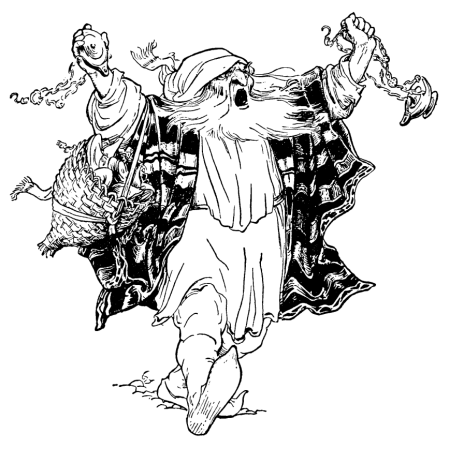
\includegraphics[scale=.5]{CivilizedArcana}
  \end{center}



\MYSTERY [
  Name = Forgehammer,
  Link = arcana-mystery-forgehammer,
  Paradigm = Force,
  Save = N,
  Duration = Session,
  Target = Self
]

A magical blacksmith's hammer appears in your hand that only you can wield.  The hammer deals \DICE+\DICE damage up to a maximum of 8. You fight with this weapon using your \FOC (instead of your \VIG).  You can repair the Max \UD of an Ally's armor during a Bivouac; for every \DCUP you repair in this way, the damage of the hammer goes down by 2. The Forgehammer can strike creatures who are only struck by magical weapons, but because there is no die to roll when dealing damage, it cannot Crit or be Fumbled.

Once the damage die is exhausted (reaches 0), the Forgehammer disappears.


\MYSTERY [
  Name = Hone,
  Link = arcana-mystery-hone,
  Paradigm = Force,
  Save = N,
  Duration = Combat or \SUM Minutes,
  Target = Close Target(s)
]

You run your hands over \DICE metal, stone, or wooden edges and hone them to a razor sharpness. If the object is a Bashing weapon, it deals +\DICE damage; if the object is a Stabbing or Chopping weapon, it deals +\DICE X2 damage. The edge must be smaller than your outstretched arms.

\MYSTERY [
  Name = Millworks,
  Link = arcana-mystery-millworks,
  Paradigm = Entropy,
  Save = N,
  Duration = Instant,
  Target = Close Target(s)
]

A tree no larger than \DICE X 5m tall and \DICE meters in diameter topples over, as if neatly cut. The result depends on the dice you invest. 1 \DICE: cut and broadly de-limbed, 2 \DICE: cut, de-limbed, debarked, 3 \DICE: cut, de-limbed, debarked, cut into planks as per your specifications, stacked, 4 \DICE cut, planed, de-limbed, debarked, cut into planks, stacked, sanded, and finished. Small limbs and offcuts will be piled for kindling. Alternatively, you can reduce the tree to sawdust or wood chips in 20-\SUMDICE minutes


\MYSTERY [
  Name = Package Neatly,
  Link = arcana-mystery-package-neatly,
  Paradigm = Entropy,
  Save = n/a,
  Duration = Concentration or Permanent,
  Target = Nearby Target(s)
]

Up to \DICE X250kg of nonliving objects, as you designate, are packed neatly. You must name the objects or their general category when you cast the spell ("those coins", "the contents of that room") If no packing materials are provided, the objects will be stacked into compact cubes, with the largest and most stable objects at the bottom. If chests, paper and twine, sacks, carts, etc. are provided, the spell will use them as you direct. The packages created will take up the minimum space possible, and will be remarkably sturdy. The spell will continue to pack objects for as long as you maintain concentration. The objects must be able to move freely. You could not use this spells to pack clothes someone was wearing. The objects will not lift more than 3m off the ground during the packing process.

\mysubsection{Cthonic}{arcana-mystery-cthonic}
\MYSTERY [
  Name = Abyssal Trident,
  Link = arcana-mystery-abyssal-trident,
  Paradigm = Force,
  Save = N,
  Duration = Session,
  Target = Self
]

A magical trident appears in your hand that only you can wield.  The trident is a 2-handed weapon that deals \DICE+\DICE damage up to a maximum of 12.   You fight with this weapon using your \FOC (instead of your \VIG).  Every time the trident deals damage, its damage goes down by 1. The trident can strike creatures who are only struck by magical weapons, but because there is no die to roll when dealing damage, it cannot Crit or be Fumbled. 

Once the damage die is exhausted (reaches 0), the Abyssal Trident disappears.

\MYSTERY [
  Name = Davy Jones's Locker,
  Link = arcana-mystery-davy-joness-locker,
  Paradigm = Prophesy,
  Save = N,
  Duration = Instant,
  Target = Close Target(s)
]

You must be near a body of water to use this liturgy (a river is OK, a puddle isn't).  You summon a chest up to \DICE meters in length, width, and height.  The box can hold up to \DICE X100kg in weight, or about 25 Significant Items (provided the box is big enough in terms of height, width, and depth i.e. you could lie a 2 meter long pole in a 2 [die] locker).  Once you seal the box and carve your name onto it, the waters will take the locker back beneath the surface, where it will disappear.  At any time, you can return to the same body of water and bring the locker back from the depths. Nothing else can bring the locker back from the deeps (not even the liturgy of Dredge) except your death.  When you die, the locker will wash up on shore within a few days for some lucky (or unlucky) soul to find.
If you place a living thing inside, it can breathe - but it will starve or die of thirst without food or water (incidentally, this is a great way to make \myital{vodyanoi})

\MYSTERY [
  Name = Dredge,
  Link = arcana-mystery-dredge,
  Paradigm = Mind,
  Save = N,
  Duration = Concentration,
  Target = Close or Nearby
]

The ground \DICE+\DICE meters in diameter (with you at the center) rumbles and quakes.  Buried or covered objects rise \DICE x5 meters to the surface.  Coins, stones, and roots will be pulled to the surface; if you cast it on water, sunken objects will rise to the surface and remain as long as you concentrate.  The objects cannot weigh more than \DICE x100kg.  

\MYSTERY [
  Name = Excavate,
  Link = arcana-mystery-excavate,
  Paradigm = Elements,
  Save = N,
  Duration = Instant,
  Target = Close
]

You can remove up to \DICE inorganic materials from a \DICE x5 meter cube just in front of your feet.  The materials could be "stone", "water", "dirt", etc. The materials disappear permanently. Objects that would be suspended in the material removed will obey the laws of physics - removing water will cause the surrounding water to rush in, removing dirt from around a chest will cause the chest to fall, etc.

\MYSTERY [
  Name = Fade,
  Link = arcana-mystery-fade,
  Paradigm = Mind,
  Save = Y (neg.),
  Duration = Markovian,
  Target = Nearby Target(s)
]

You can cause a Ally, Monster, or object to fade out of existence.  You can still see them, though they're insubstantial (like a ghost).  The target can't move, talk, or interact with the world in any way.  Not even magic can affect the target.  If the target is unwilling, it gets a Save to negate.  The duration is Markovian and depends on the number of \DICE invested.

  \begin{center}
  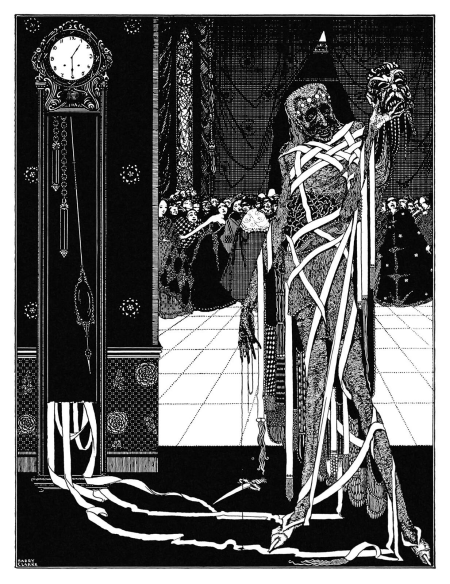
\includegraphics[scale=.5]{CthonicArcana}
  \end{center}


\MYSTERY [
  Name = Mermaid's Breath,
  Link = arcana-mystery-mermaids-breath,
  Paradigm = Biomancy,
  Save = Y (neg.),
  Duration = \SUM Minutes,
  Target = Self or Close Target(s)
]

For \SUMDICE Minutes, up to \DICE+1 Allies or Monsters (including yourself) can breathe water as if it were air.  They can only breathe water, however - breathing air will cause them to drown. Unwilling creatures get a Save to negate.  You must touch the Creature to bestow this mystery upon them. 

\MYSTERY [
  Name = Sinister Stillness,
  Link = arcana-mystery-sinister-stillness,
  Paradigm = Mind,
  Save = N,
  Duration = Combat or \SUM Minutes,
  Target = Close\, Nearby\, Far-Away\, or Distant
]

You can invoke this liturgy in an area  Close, Nearby, Far-Away, or Distant from yourself.  The air Close to the area takes on an unsettling air of silence.  Sound is not magically suppressed, but Monsters and creatures within its bounds feel that any sound they make will disturb something better left undisturbed.  Non-intelligent animals will not enter the area, and Monsters inside must make an immediate morale check. Thereafter, Saves against fear effects have a -\DICE and morale rolls suffer a -\DICE penalty (maximum -4).  A morale check is needed to enter or pass through the area of the spell.

\MYSTERY [
  Name = Sound the Deeps,
  Link = arcana-mystery-sound-the-deeps,
  Paradigm = Force,
  Save = N,
  Duration = Instant,
  Target = Close Target(s)
]

You slap your hand on the ground or the surface of the water.  The echoes of the tremor allow you to precisely know how deep and the approximate shape of bodies of water, chasms, shafts, clefts, mountain peaks, caverns, passages, etc.  up to a distance of \DICE x100m meters.  Additionally, you may use this to rouse \DICE+\DICE Allies Close, Nearby, Far Away, or Distant who are Sleeping, Knocked Out, etc. 

\newpage

\mysubsection{Cunning}{arcana-mystery-cunning}
\MYSTERY [
  Name = Expertise,
  Link = arcana-mystery-expertise,
  Paradigm = Mind,
  Save = N,
  Duration = \SUM Minutes,
  Target = Self
]

Name a Skill - it can be one of the 7 basic skills, or any other skill you choose (though you can't learn things that would not be contained in a well stocked library, or that are so rare that only a few people could teach them to you).  You are Skilled (d12+2) in that Skill for the spell's duration.  If you already know the Skill at a level of Skilled or better, add +\DICE x2 (up to a maximum of +4) to your Skill roll.

\MYSTERY [
  Name = Illusion,
  Link = arcana-mystery-illusion,
  Paradigm = Mind,
  Save = N,
  Duration = Varies,
  Target = See Below
]

You create an illusion of anything you desire. If anything touches the illusion, it will pass through it with no effect.  The illusion cannot be greater than \DICE x \DICE meters in size.  Think of the illusion as a perfectly accurate hologram that you are creating - the illusion can be heard in addition to being seen, can perform the same action over and over again, and can deliver messages, but it can't interact in a meaningful way or perform complex actions based on external forces. 

Each aspect of the illusion requires one or more Faith to cast:

\mybullet {
  \item You want the illusion to say up to \DICE + \DICE words or make \DICE + \DICE sounds (wailing, shouting, etc)
  \item You want the illusion to be a physical thing (hole in the ground, stone wall, orc guard, etc)
  \item You want the illusion to be able to move up to \DICE meters
  \item You want to cast the illusion on a living creature (disguise them as a beggar or a lamp post)
}

Note that there is some Arbiter's discretion here.  A guard pacing in front of a door might cost 2 \DICE (a physical thing moving back and forth 2
meters), but if you want the illusion of acrobats or pouncing lions it will be more costly.  A disguise cast on someone to appear to be a beggar might
cost 1 [die] (a living creature wearing the face and clothing of a random beggar), but disguising yourself as the king will be significantly harder.

The Illusion will last for \DICE Hours.  Anyone touching the illusion will immediately know it to be fake, but this doesn't cause the illusion to
disappear.  However, if the illusion is touched with an \mylink{Ego Weapon}{wizardry-ego-weapon}, it will immediately evaporate.

\MYSTERY [
  Name = Labyrinth,
  Link = arcana-mystery-labyrinth,
  Paradigm = Mind,
  Save = N,
  Duration = Combat or \SUM Minutes,
  Target = Self
]

You create a spiraling labyrinth of thought in your mind.  Anyone targeting you with Charm, Sleep, or any magical effect where the caster tries to read your mind or alter your memories must enter into a \RB : \FOC contest with you at a -\DICE penalty.  If they fail, they will be caught in your mind for the duration of the spell;  their physical body immediately catches the Vapors, and you can hear all their thoughts.

  \begin{center}
  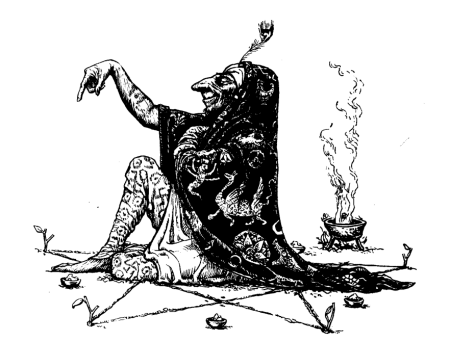
\includegraphics[scale=.5]{CunningArcana}
  \end{center}



\MYSTERY [
  Name = Memory Lane,
  Link = arcana-mystery-memory-lane,
  Paradigm = Mind,
  Save = Y (neg.),
  Duration = Varies,
  Target = Close Target(s)
]

You can create a memory (real or not) and embed it in the head(s) of up to \DICE creatures by touch.  Unwilling creatures may Save to negate the spell.  The memory must be short and distinct.  The memory will start to fade in a few days, but if you win a \RB : \FOC attempt against the victim (the victim has a -\DICE penalty) when you invoke the mystery, the memory will never fade, even if they lose all other memories (incidentally, this is is a really great way to create a ghost or poltergeist).

\MYSTERY [
  Name = Mirror Image,
  Link = arcana-mystery-mirror-image,
  Paradigm = Mind,
  Save = n/a,
  Duration = Minutes,
  Target = Self
]

You create \DICE illusory images of yourself, which move as you move and always stay Close to you. They are constantly stepping through each other, so that it is impossible to tell which is which. When an enemy attacks you, roll to see if they hit you or an image (equal chance). An image vanishes as soon as it suffers a solid impact (a blow from a mace, but also a slap). Area effects such as a dragon's breath will cause all images to instantly vanish (and you'll take fire breath damage, naturally).

\MYSTERY [
  Name = Paralysis,
  Link = arcana-mystery-paralysis,
  Paradigm = Mind,
  Save = Y (neg.),
  Duration = Markovian,
  Target = Close or Nearby Target(s)
]

Up to \DICE creatures of \DICE \HD or less must Save or be Paralyzed.  Sleeping creatures do not get a Save. The duration is Markovian and depends on the number of \DICE invested

\MYSTERY [
  Name = Strange Copy,
  Link = arcana-mystery-strange-copy,
  Paradigm = Mind,
  Save = N,
  Duration = \SUM Hours,
  Target = Close Target(s)
]

You reach into a mirror-like surface and pull out a copy of an object reflected in the mirror. The object that you pull out must be within reach of the mirror (as if it were a window), small enough to fit through the mirror (as if it were a window) and can't weigh more than \DICE x10kg. The mirror object looks and feels exactly like the object it copied, though it is a mirror image (so if you were to copy a book, the text would be backwards).  You can't copy any magical properties of the object, and you can only duplicate objects, not living things.  The object exists for \SUMDICE Hours.  If the object suffers a solid blow, it pops like a bubble.

\MYSTERY [
  Name = Twin,
  Link = arcana-mystery-twin,
  Paradigm = Mind,
  Save = N,
  Duration = \SUM Minutes,
  Target = Close Target(s)
]

You reach into a mirror-like surface and pull out a copy of yourself.  The mirrored surface has to be big enough for you to walk through - same height and same width, at least.  The copy behaves just like you, but it's illusory - anything that touches it will pass right through it, and it can't pick anything up or hold anything.  You can switch places with your mirror-self by stepping through the mirror - this dispels the illusion, and you appear wherever your mirror self is at the moment you step through.

\newpage

\mysubsection{Empyrean}{arcana-mystery-empyrean}
\MYSTERY [
  Name = Children of Shul,
  Link = arcana-mystery-children-of-shul,
  Paradigm = Prophesy,
  Save = Y (half),
  Duration = Session,
  Target = Self
]

You create \DICE small moons that circle the top of your head, casting moonlight Close and Nearby.  The shadows thrown by this moonlight give a +\DICE bonus (up to +4) to all Whispers made by Allies who are Close to you.  The moonlight will also activate abilities and powers that manifest in lunar rays (like lycanthropy), and throw light equivalent to \DICE x10 candles.

You can unerringly throw one these moons at Nearby Monsters every Moment, striking for 4 damage each (including creatures only struck by Magic weapons).  When you have no moons left, the spell ends.

The moons can be dispelled at any time, but can only be summoned once a Session.

\MYSTERY [
  Name = Glorious Sunburst,
  Link = arcana-mystery-glorious-sunburst,
  Paradigm = Elements,
  Save = Y (half),
  Duration = Combat or \SUM Minutes,
  Target = See Below
]

You raise your hands to the heavens and fire a flare up to 50m upwards, where it hovers providing bright sunlight to all areas Close, Nearby, and Far-Away.  You can command the sunburst to change color, move horizontally, or explode.  No shadows can be cast beneath the sunlight (meaning sneaking around is difficult if not impossible), and all invisible creatures and objects appear with a thin halo around them the color of the sun.  Anyone who performs the sacrament Curse the Unhallowed while under the Glorious Sunburst adds an additional +\DICE x2 to their damage; anyone Close to the sunburst if it explodes takes \SUMDICE+\DICE damage, Save for half.

\MYSTERY [
  Name = Lightning,
  Link = arcana-mystery-lightning,
  Paradigm = Elements,
  Save = Y (half),
  Duration = Instant,
  Target = Close or Nearby Target(s)
]

Forks of lightning erupt from your forehead, striking a Close or Nearby target for \SUMDICE+\DICE damage (Save for half). You can cause the lightning to "jump" up to \DICE-1 times to another creature or object Close by, provided they are conductive (iron armor, metal ladders, etc).  Magic swords aren't conductive.  You can "ping-pong" between two objects if you desire. Creatures struck by a secondary (or greater) lightning bolt take \DICE damage (no Save). Objects struck by the lightning bolt will become momentarily electrified, and deal a shock that could cause someone to lose their grip unless they \RO : \VIG + \FOC with a -\DICE penalty.

\MYSTERY [
  Name = Lunacy,
  Link = arcana-mystery-lunacy,
  Paradigm = Mind,
  Save = Y (neg.),
  Duration = Markovian,
  Target = Close or Nearby Target(s)
]

You invoke the madness of the moon.  \DICE creatures must immediately \RS : Sanity; if they do not have Sanity (Monsters, for instance) the creatures are permitted a Save.

The Lunacy is random for each Monster that fails its Save.  Roll a d4:  1) the Monster becomes Enraged at someone or something that isn't an Ally; 2) the Monster becomes Afraid of you and your Allies; 3) the Monster is Knocked Out; 4) the Monster suffers Anathema.  The duration is Markovian and depends on the number of \DICE used.

  \begin{center}
  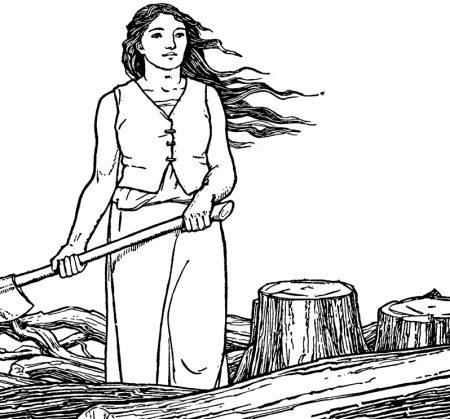
\includegraphics[scale=.5]{EmpyreanArcana}
  \end{center}


\MYSTERY [
  Name = Mountainhands,
  Link = arcana-mystery-mountainhands,
  Paradigm = Biomancy,
  Save = N,
  Duration = Session,
  Target = Self
]

Your hands enlarge and become stone.  Unarmed Attacks do +\DICE damage (up to a maximum of +4).  In addition, you can reach your hands into substances that might affect Flesh but not stone (fire, boiling water - OK.  Lava or acid - not OK).  Holding a stone in your hands allows you to speak to it as the Murk ability (see the Core Rules). 

Your hands must be empty (including rings and gloves) in order to invoke this mystery. You can only invoke this mystery once per Session.

\MYSTERY [
  Name = Rainburst,
  Link = arcana-mystery-rainburst,
  Paradigm = Elements,
  Save = n/a,
  Duration = Combat or \SUM Minutes,
  Target = See Below
]

You create a rainstorm in the surrounding area.  The rain extinguishes all fires (even magical ones) for the duration, prevents non-magical fires from starting, and heals Allies and Monsters alike for \SUMDICE Flesh (once at the moment of invocation).  The range is dependent on the number of \DICE invested: 1 Close; 2-3 Close and Nearby; 4-6 Close, Nearby, and Far-Away; 7+ Close, Nearby, Far-Away, and Distant.

\MYSTERY [
  Name = Resonating Command,
  Link = arcana-mystery-resonating-command,
  Paradigm = Mind,
  Save = Y (neg.),
  Duration = Markovian,
  Target = Nearby Target(s)
]

You shout a one word command at up to \DICE Close or Nearby target, who must obey (Save negates).  The target(s) must be able to understand your language.  The command resonates for a Markovian duration - if the Markovian die is not a 1 or a 2, they must Save again.  Each Moment after the first the target(s) gain an additional +1 to their Save.  The command cannot directly cause the target(s) harm or force them to commit a harmful action.  You could cause them to run into a trap they didn't know was there, or into a tactically disadvantageous position, but not off a cliff.

\MYSTERY [
  Name = Thunderclap,
  Link = arcana-mystery-thunderclap,
  Paradigm = Elements,
  Save = Y (neg.),
  Duration = Instant,
  Target = Far-Away or Distant
]

You can invoke this mystery somewhere Far-Away or Distant from yourself.  Monsters Close to the Thunderclap must immediately make a morale check with a -\DICE penalty, or become Afraid of you.  Additionally, Monsters become Deafened for \DICE Moments unless they make a Save with a -\DICE penalty.

\newpage

\mysubsection{Errant}{arcana-mystery-errant}
\MYSTERY [
  Name = Armor of Winds,
  Link = arcana-mystery-armor-of-winds,
  Paradigm = Entropy,
  Save = n/a,
  Duration = Session,
  Target = Self
]

Take \DICE Faith and put them "in reserve".  For the remainder of the Session, you may sacrifice one of these [die] to cause any single \mybold{physical} attack that would damage you to miss instead of hit.  You must sacrifice the [die] \myital{before} you roll your Guard or Save.  You can only use 1 [die] per Moment.  Any unused \DICE are lost at the end of the Session.  You can only invoke this mystery once per Session.

\MYSTERY [
  Name = Capture Wind,
  Link = arcana-mystery-capture-wind,
  Paradigm = Elements,
  Save = N,
  Duration = Concentration or Session,
  Target = See Below
]

A magical circle \DICE meters in radius extends from your fingertip in front of you. As long as you maintain concentration, you can absorb any wind passing through the circle. You can then collapse the spell. 

At any time during the Session, you can reactivate the circle to release the wind you absorbed.  The wind flows out at the same rate it entered. If you activate this spell in a light breeze for 5 minutes, the spell will release a light breeze over 5 minutes. The wind only flows from the circle, so anyone standing behind it is not affected (unless you release hurricane-force winds indoors). You can cancel the release at any time, which expends the spell as usual. If you go to 0 Flesh while the spell is still "reserved", it immediately activates facing a random direction.  

If the wind is a magical breath that would do damage (dragon's breath, etc.) your \SUMDICE must be equal to or greater than the sum of the damage, or the circle immediately collapses.  

\MYSTERY [
  Name = Corsair's Blade,
  Link = arcana-mystery-corsairs-blade,
  Paradigm = Force,
  Save = n/a,
  Duration = Session,
  Target = Self
]

A magical rapier appears in your hand that only you can wield.  The rapier deals \DICE+\DICE damage up to a maximum of 6.  You must make a successful Fight check using your \FOC (instead of \VIG or \DEX).  The Hero's Rapier ignores Armor and Soak, and while you wield it you always win Init. The rapier can strike creatures who are only struck by magical weapons, but because there is no die to roll when dealing damage, it cannot Crit or be Fumbled.  


  \begin{center}
  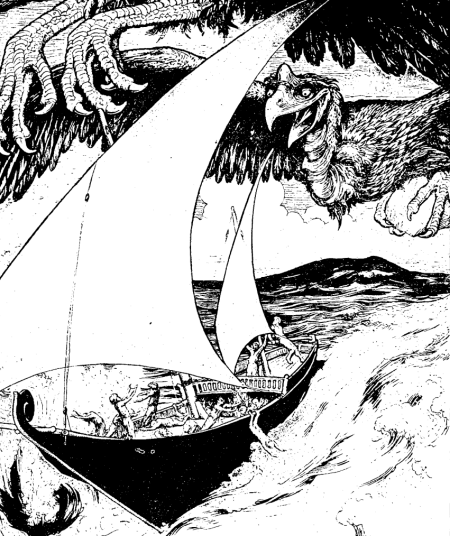
\includegraphics[scale=.5]{ErrantArcana}
  \end{center}



\MYSTERY [
  Name = Duelists' Wings,
  Link = arcana-mystery-duelists-wings,
  Paradigm = Biomancy,
  Save = n/a,
  Duration = Combat or \SUM Minutes,
  Target = Self or Close Target(s)
]

Tiny white wings sprout from the ankles and wrists of up to \DICE Allies.  They always win Init in Combat, and any falling damage is reduced by -\DICE per die.

\MYSTERY [
  Name = Ropework,
  Link = arcana-mystery-ropework,
  Paradigm = Entropy,
  Save = N,
  Duration = \SUM Minutes,
  Target = Close Target(s)
]

You summon a rope \DICE x50m in length.  You can command the rope to arrange itself into any shape and rise into the air in any orientation.  It can be climbed like a normal rope, and can support \DICE x100kg of weight.  Its ends do not need to be anchored to anything.

\MYSTERY [
  Name = Shatter Bonds,
  Link = arcana-mystery-shatter-bonds,
  Paradigm = Force,
  Save = n/a,
  Duration = Instant,
  Target = Close or Nearby
]

By invoking this mystery, you can sunder up to \DICE+\DICE bonds either Close or Nearby.  The bonds may be physical (shackles, chains, or locks) or mental (Charm, Command, Labyrinth, etc) at the Arbiter's discretion.

\MYSTERY [
  Name = Skald's Tongue,
  Link = arcana-mystery-skalds-tongue,
  Paradigm = Entropy,
  Save = n/a,
  Duration = Breather or Bivouac,
  Target = Close Target(s)
]

This mystery can only be invoked during a Breather or Bivouac.  You play a rousing song, recite part of an epic, or sing an ancient ballad.  You can heal up to \SUMDICE+\DICE Grit among all Allies who listen, divvied up any way you want.

\MYSTERY [
  Name = Vaulting Step,
  Link = arcana-mystery-vaulting-step,
  Paradigm = Force,
  Save = N,
  Duration = Instant,
  Target = Self
]

Your next \DICE+\DICE strides (about 1m each stride) land on a plane of Force the size of your foot.  The step can be taken in any direction up, down, sideways, or across (though you cannot pass through physical objects).  You can combine these in any way you want - stride 45 degrees into the air, take another step up, and a final step down (for example).  Your final step must be on a solid surface, or you fall. 


\mysubsection{Heathen}{arcana-mystery-heathen}
\MYSTERY [
  Name = Barkskin,
  Link = arcana-mystery-barkskin,
  Paradigm = Biomancy,
  Save = Y (neg.),
  Duration = Combat or \SUM Minutes,
  Target = Self or Close Target(s)
]

You or a creature you target is covered in heavy bark.  Weight is increased by \DICE x100kg and all physical damage is reduced by -\DICE for the duration of the spell, but you can't swim, jump, or run. If invoked on something already in deep water, mud, etc. the target will immediately sink at x\DICE the normal rate. Unwilling creatures get a Save to negate. 

\MYSTERY [
  Name = Bloodvine,
  Link = arcana-mystery-bloodvine,
  Paradigm = Biomancy,
  Save = N,
  Duration = Instant,
  Target = Close or Nearby Target(s)
]

This spell can only be used on a Monster who suffering from the Bleeding effect.  Vines erupt from the Monster's wounds, dealing \SUMDICE+\DICE damage (no Save).  If the damage kills the Monster, their corpse is entirely consumed in a bramble of vines

\MYSTERY [
  Name = Butterfly Hurricane,
  Link = arcana-mystery-butterfly-hurricane,
  Paradigm = Biomancy,
  Save = Y (neg.),
  Duration = Combat or \SUM Minutes,
  Target = Self
]

A whirling brightly colored mass of butterflies springs into being around you, cloaking you and anyone else Close to you.  Any ranged attacks fired into or out of the hurricane automatically miss (AoE effects like dragon's fire aren't affected).  Anyone inside of the hurricane must Save or become Befuddled for as long as they remain inside - you and up to \DICE Allies are immune.

\MYSTERY [
  Name = Clearwater,
  Link = arcana-mystery-clearwater,
  Paradigm = Elements,
  Save = n/a,
  Duration = Instant,
  Target = Self or Close Target(s)
]

This mystery can only be invoked during a Breather or a Bivouac.  You create \DICE draughts of cold, clear water that have one of the following effects:

\mynumlist {
    \item Restore \DICE Flesh
    \item Restore \SUMDICE Grit
    \item Immediately end the effect of a Toxin
    \item Immediately end the effect of a Disease
}

\MYSTERY [
  Name = Elemental Spray,
  Link = arcana-mystery-elemental-spray,
  Paradigm = Elements,
  Save = Y (half),
  Duration = Instant,
  Target = Close or Nearby Target(s)
]

You emit \DICE sprays of elements from your fingertips that you can split among \DICE Monsters.  For each Monster, if the \SUMDICE of the \DICE targeting the Monster is greater than the Monster's \HD, they take \DICE+\DICE fire damage.  If the \SUMDICE is twice the Monster's \HD or more, they also take \DICE+\DICE cold damage.  If the \SUMDICE is three times the Monster's \HD or more, they also take \DICE+\DICE lightning damage.  If the \SUMDICE is four times the Monster's \HD or more, they also take \DICE+\DICE acid damage.  Save for half.

\MYSTERY [
  Name = Entangling Smoke ,
  Link = arcana-mystery-entangling-smoke,
  Paradigm = Elements,
  Save = Y (neg.),
  Duration = Markovian,
  Target = Close or Nearby Target(s)
]

This spell requires the Narcotic: Pipeweed.  You breathe out a plume of smoke; up to \DICE creatures or objects are grabbed by tendrils of this smoke unless they Save.  Those who fail move at half speed (meaning it takes 2 Maneuvers to move somewhere Nearby; for Monsters, it means their speed is Slow if it isn't already).  Any Ally fighting this Monster gains a +\DICE bonus to Fight and Guard. The duration is Markovian and depends on the number of \DICE invested.

\MYSTERY [
  Name = Hearthfire,
  Link = arcana-mystery-hearthfire,
  Paradigm = Elements,
  Save = n/a,
  Duration = Bivouac,
  Target = Close Target(s)
]

During a Bivouac, you may perform up to \DICE effects, once per die (though you may choose an effect multiple times):
\mybullet {
\item Repair the \MAX \UD of an Allies armor to full
\item Provide Provisions for 1 Ally
\item Heal up to \DICE Flesh on 1 Ally
\item Prevent any Wandering Monsters from attacking your camp
}

  \begin{center}
  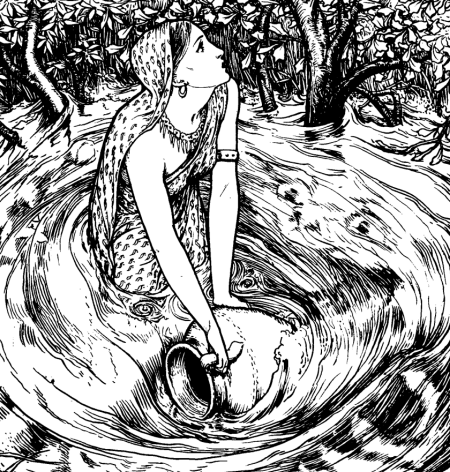
\includegraphics[scale=.5]{HeathenArcana}
  \end{center}



\MYSTERY [
  Name = Sporous Breath,
  Link = arcana-mystery-sporous-breath,
  Paradigm = Biomancy,
  Save = Y (neg.),
  Duration = Combat or \SUM Minutes,
  Target = Nearby Target(s)
]

You breathe a cloud of mushroom spores into an area Nearby.  All Allies and Monsters are affected by the Sporous Breath unless they make their Save.  The effects depend on the number of \DICE used: 1) all targets suffer Anathema; 2-3)  all targets are Woozy; 4-5 all targets are Befuddled; 6+) all targets are affected with an Iron (d4) Toxin.

Only yourself and Pooka are immune to the effects of the Sporous Breath.

\mysubsection{Jötnar}{arcana-mystery-jötnar}
\MYSTERY [
  Name = Dirge,
  Link = arcana-mystery-dirge,
  Paradigm = Death,
  Save = n/a,
  Duration = Concentration,
  Target = Close Target(s)
]

You begin droning a hero's dirge.  For as long as you concentrate, all Close and Nearby Allies gain a +\DICE bonus to their \DEATH checks, up to a maximum of +4.

\MYSTERY [
  Name = Extinguish,
  Link = arcana-mystery-extinguish,
  Paradigm = Elements,
  Save = N,
  Duration = Instant,
  Target = Close or Nearby Target(s)
]

Beams of slushy ice shoot from your outstretched hands and strike up to \DICE+\DICE targets.  Multiple beams can hit the same target.  If the target is on fire, the flame is immediately extinguished.  Flames the size of torches only require 1 [die]; people or animals would require 2 \DICE; bonfires and the like require 3+ \DICE at the Arbiter's discretion.

\MYSTERY [
  Name = Giantform,
  Link = arcana-mystery-giantform,
  Paradigm = Biomancy,
  Save = n/a,
  Duration = Combat or \SUM Minutes,
  Target = Self
]

You grow \DICE x 500cm in height, with strength to match.  Your Unarmed Attacks do an extra point of damage for every 2 \DICE you spend, and you can lift an additional \DICE x100kg.   If you are wearing Armor when you invoke Giantform, you take \MAX \UD in Flesh damage, and the Armor is ruined (drops to 0 \MAX \UD).  You are unable to use "normal" sized weapons while in Giantform.

\MYSTERY [
  Name = Incinerate,
  Link = arcana-mystery-incinerate,
  Paradigm = Elements,
  Save = N,
  Duration = See Below,
  Target = Close Target(s)
]

This mystery requires you to create a bonfire.  You can place up to \DICE inorganic objects into the fire weighing no more than \SUMDICE kg.  The objects are burned to a pile of enchanted ash, which can be harvested and stored as an Insignificant item.  When you wish the objects to become whole again, you must build a fire and sprinkle the ash inside of it; you can reach into the fire unharmed to pull the objects from the flames as they were when you placed them into the fire.  If you perish before the objects are retrieved, the ash reverts to normal, unenchanted ash and the objects are destroyed.


  \begin{center}
  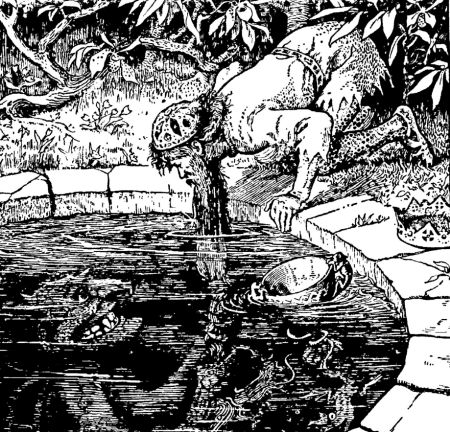
\includegraphics[scale=.5]{JotnarArcana}
  \end{center}



\MYSTERY [
  Name = Preserve,
  Link = arcana-mystery-preserve,
  Paradigm = Elements,
  Save = Y (neg.),
  Duration = varies,
  Target = Close Target(s)
]

By touching an object, you are able to freeze it for a period of time in order to preserve it.  If the object is an Ally or Monster, they must be lying completely still in order to use the liturgy.  Unwilling creatures get a Save.  While frozen, any toxins, diseases, bleeding, or negative effects are stopped for a period of time, depending on the number of dice spent.  You cannot end this liturgy willingly once it has begun, though it could be ended prematurely by great heat (a very large bonfire, for example) or by taking more than \SUMDICE points of damage, which will cause the object to shatter into many pieces.  

1 [die]: Minutes; 2-3 \DICE: Days; 4-5 \DICE: Weeks; 4 \DICE: Months; 6-7 \DICE: Years; 8+ \DICE: Permanent. 

\MYSTERY [
  Name = Ray of Fire,
  Link = arcana-mystery-ray-of-fire,
  Paradigm = Elements,
  Save = Y (neg.),
  Duration = Instant,
  Target = Nearby or Far-Away Target(s)
]

A narrow beam of fire shoots from your outstretched finger.  Make a Fight roll using your \FOC with a +\DICE modifier (up to +4); if you hit, the target catches fire for a Markovian duration if they fail a Save.  They are only allowed 1 Save.  They damage taken by the target is whatever is rolled on the Markovian die each Moment.  The beam of fire will also light flammable things alight.

\MYSTERY [
  Name = Trollblood,
  Link = arcana-mystery-trollblood,
  Paradigm = Death,
  Save = n/a,
  Duration = Combat,
  Target = Self
]

This mystery can be invoked at any time during Combat.  As long as you are alive, you regenerate +\DICE Flesh at the bottom of each Moment.  This regeneration is negated if the damage is from an acid or fire source. At the end of Combat, this mystery immediately ends (before you can take a Breather).

\MYSTERY [
  Name = Witness Me,
  Link = arcana-mystery-witness-me,
  Paradigm = Death,
  Save = n/a,
  Duration = Combat,
  Target = Self
]

This mystery can only be invoked in Combat.  For the remainder of Combat, you gain +\DICE x2 (up to +8) on your Fight checks, and deal +\SUMDICE damage when you hit (rolled each time along with your damage).  At the end of Combat, you immediately catch the Vapors and drop to 0 Flesh, and must make a \DEATH check.

\newpage

\mysubsection{Monstrous}{arcana-mystery-monstrous}
\MYSTERY [
  Name = Dragonbreath,
  Link = arcana-mystery-dragonbreath,
  Paradigm = Elements,
  Save = Y (half),
  Duration = Instant,
  Target = Nearby
]

You breathe out a gout of dragon's breath before you.  The breath deals \SUMDICE+\DICE damage to all creatures Nearby, Save for half damage (plus see below).  The type of breath is random, roll a d6 for the type of breath: 1) Fire (Red); 2) Acid (Black); 3) Frost (White); 4) Lightning (Blue); 5) Corrosive Gas (Green); 6) Void (Bone).  The additional effect of the dragon's breath is as follows:

\mybullet {
  \item \mybold{Red:}   Fire.  If you fail your Save, you catch fire.  Take d4 damage at the top of each Moment until you spend an entire Moment doing "stop, drop, and roll".  This can be shortened to a single Maneuver if someone helps you.
  \item \mybold{Black:}  Acid.  If you fail your Save, take d4 acid damage for d4 Moments
  \item \mybold{White:}  Frost.  If you fail your Save, you are knocked Prone
  \item \mybold{Blue:}  Lightning.  If you fail your Save \mybold{and} are wearing metal armor, take an additional 1 point of damage per die
  \item \mybold{Green:}  Corrosive gas.  If you fail your Save, reduce your Soak by 1, or roll your  Armor \UD
  \item \mybold{Bone:}  Void.  If you fail your Save, you catch the Vapors for d4 Markovian
}

\MYSTERY [
  Name = Harpy's Talons,
  Link = arcana-mystery-harpys-talons,
  Paradigm = Force,
  Save = n/a,
  Duration = Session,
  Target = Self
]

Your fingers sprout iron-hard talons.  The talons can strike for \DICE damage each up to a maximum of 4.  You can strike with both of these Talons in Combat at the same time; roll your Fight die twice using your \FOC (instead of your \VIG).  If both talons hit, the Monster is also afflicted with Bleeding.  Every time your talons deal damage, their damage goes down by 1 (you tell the Arbiter which Talon goes down in damage, either "left" or "right"); when \mybold{one} of the Harpy's Talons hits 0 damage, the talon disappears (you can still strike with the other talon, but it won't have the Bleeding effect). The talons can strike creatures who are only struck by magical weapons, but because there is no die to roll when dealing damage, it cannot Crit or be Fumbled

\MYSTERY [
  Name = Serpent's Fang,
  Link = arcana-mystery-serpents-fang,
  Paradigm = Biomancy,
  Save = n/a,
  Duration = Combat or \SUM Minutes,
  Target = Self
]

Make your Fight \RO using your \FOC.  If you succeed, you grapple a Monster and may immediately bite them with your fangs.  The Monster takes \DICE damage and begins Bleeding, unless they Save.  You may apply Toxins to your fangs, but if you do so you must \RS : \FOC or accidentally ingest the Toxin, with the appropriate negative effects.

\MYSTERY [
  Name = Slimeform,
  Link = arcana-mystery-slimeform,
  Paradigm = Biomancy,
  Save = n/a,
  Duration = \SUM Minutes,
  Target = Self
]

You transform yourself and all of your Gear into a slime.  You can absorb up to \SUMDICE+\DICE damage without any ill effects (damage after this goes straight to Flesh, and immediately ends the mystery).  You are unable to attack, talk, cast spells, etc while in Slimeform, but you can move at a the pace of a slow walk, climb walls, hang from the ceiling, and slip under the cracks of doors if you wish.

\MYSTERY [
  Name = Spidertongue,
  Link = arcana-mystery-spidertongue,
  Paradigm = Biomancy,
  Save = Y (neg.),
  Duration = Combat or \SUM Minutes,
  Target = Self
]

You can speak with spiders (and they can speak with you).  Small spiders know about water, wind, and bugs.  Larger spiders know about people (maybe they can tell them apart).  Big, dangerous spiders know all kinds of things.  Spiders will be friendly towards you, but if you attack them they'll fight back.  Additionally, your spittle becomes a Toxin whose power depends on the number of \DICE spent: 1-2 \DICE Iron Toxin; 3-4 \DICE Silver Toxin; 5+ \DICE Gold Toxin.  Your spittle is enough to poison a drink, a needle or syringe, or infect someone you might bite, but not enough to poison a knife or dagger.  The spittle becomes normal when the duration ends.


  \begin{center}
  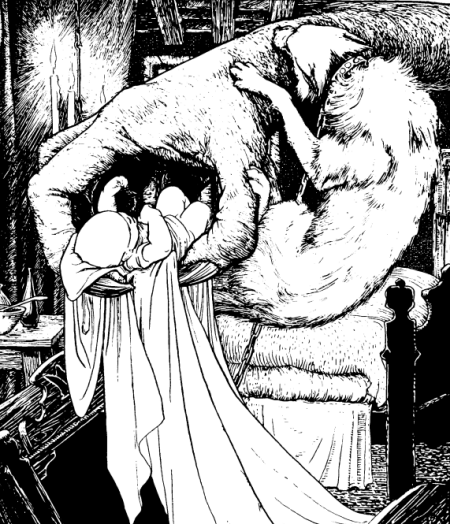
\includegraphics[scale=.5]{MonstrousArcana}
  \end{center}


\MYSTERY [
  Name = Tasty,
  Link = arcana-mystery-tasty,
  Paradigm = Biomancy,
  Save = N,
  Duration = Combat or \SUM Minutes,
  Target = Close Target(s)
]

The target object or Monster (alive or dead) smells delicious for the spell's duration.  The smell radiates Nearby in calm air, but can spread on the wind, or leave a trail.  Non-intelligent zoological creatures and swarms will be attracted to and attempt to eat the object or Monster first (even if they are supposed to be allies); intelligent creatures get a Save at a -\DICE penalty. 

\MYSTERY [
  Name = Tattered Robe,
  Link = arcana-mystery-tattered-robe,
  Paradigm = Entropy,
  Save = Y (neg.),
  Duration = Combat or \SUM Minutes,
  Target = Self
]

You must be wearing robes without armor to use this liturgy.  The edges of your robes form into \DICE tatters, each of which can be used as a weapon in combat in addition to your regular attack. The tatters deal no damage and each of their attacks must be rolled separately using your \FOC instead of your \VIG or \DEX - but if you hit the target begins Bleeding unless they make a Save.  You can split these attacks among as many Close opponents as you desire.

The tatters can also be used to hold small objects, as if they were each a prehensile tail.  Each tatter can hold up to 5kg of weight, but cannot attack if they are holding something.

\MYSTERY [
  Name = Undead Visage,
  Link = arcana-mystery-undead-visage,
  Paradigm = Death,
  Save = n/a,
  Duration = Combat or \SUM Minutes,
  Target = Self
]

You turn yourself into a hideous undead caricature of your "normal self".  You immediately become Unhallowed and gain the following effects, based on the number of \DICE spent:  1-2 you are immune to spells from the Mind Paradigm; 3-4 you are immune to Toxins; 5-6 you are immune to spells of the Force paradigm; 7+  you are immune to iron weapons.  These effects are cumulative.

You can only speak Graveborn for the duration of the spell.  Your Undead form prompts a Sanity or morale check among all who see you (Allies and Monsters alike), unless they have seen you in your Undead form before. 


\mysubsection{Righteous}{arcana-mystery-righteous}
\MYSTERY [
  Name = Crusader's Helm,
  Link = arcana-mystery-crusaders-helm,
  Paradigm = Force,
  Save = n/a,
  Duration = Session,
  Target = Self
]

You summon an ivory basinet, complete with crest, neck guard, and visor.  While worn, the Crusader's Helm protects you as a normal helmet (ignore certain Physical Wounds, etc), and you can absorb up to \DICE spells of the Mind paradigm without effect.  With the visor down you can detect Invisible creatures and are immune to Surprise (including the Drop).

\MYSTERY [
  Name = Grounding Mantra,
  Link = arcana-mystery-grounding-mantra,
  Paradigm = Elements,
  Save = Y (neg.),
  Duration = Markovian,
  Target = Close\, Nearby\, or Far-Away Target(s)
]

By invoking this liturgy, you shackle up to \DICE creatures to the ground.  They must be touching the ground already when you make the invocation.  The creatures must keep at least one limb touching the ground at all times.  If they attempt to run, they must \RB : \DEX with a -\DICE penalty.  If they are knocked Prone, they must \RB : \VIG with a -\DICE penalty to stand up.  Save negates.

\MYSTERY [
  Name = Holy Weapon,
  Link = arcana-mystery-holy-weapon,
  Paradigm = Force,
  Save = n/a,
  Duration = Session,
  Target = Self
]

A holy weapon (describe to the Arbiter) appears in your hands that only you can wield.  The weapon is a 2-handed weapon that deals \DICE+\DICE damage up to a maximum of 10.  In addition, you deal +\DICE damage against Unhallowed creatures. You fight with this weapon using your \FOC (instead of your \VIG). Every time the weapon deals damage, its damage goes down by 1; when it hits 0, the weapon disappears.  The Holy Weapon can strike creatures who are only struck by magical weapons, but because there is no die to roll when dealing damage, it cannot Crit or be Fumbled. 

\MYSTERY [
  Name = Purging Fire,
  Link = arcana-mystery-purging-fire,
  Paradigm = Elements,
  Save = N,
  Duration = \SUM Minutes,
  Target = See Below
]

This mystery requires you to create a bonfire.  Up to \DICE Allies can step into the flames of the Purging Flames; each Moment they remain inside of the fire; they take 2 damage to Flesh, but can activate 1 of the following effects:

\mynumlist {
    \item Immediately end a Markovian effect;
    \item Immediately remove a Curse;
    \item Immediately remove a non-serious Spiritual wound;
    \item Immediately purge a Toxin
}

Anyone inside of the Purging Flames cannot lie, and must answer truthfully any question asked of them


  \begin{center}
  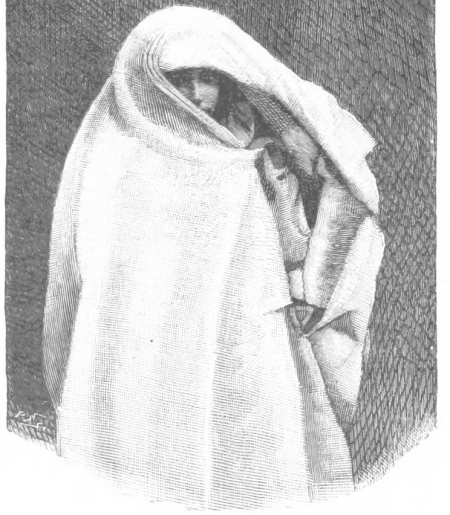
\includegraphics[scale=.5]{RighteousArcana}
  \end{center}



\MYSTERY [
  Name = Revered Aegis,
  Link = arcana-mystery-revered-aegis,
  Paradigm = Force,
  Save = n/a,
  Duration = Session,
  Target = Self
]

Take \DICE Faith and put them "in reserve".  You summon a brightly mirrored shield that can be Splintered (see the Combat Actions under Core Rules) up to \DICE times before it disappears.  Note that Splintering your shield is a Combat Action, and it ends your Moment; conversely, if you already took a Combat Action this Moment, you can’t Splinter the Revered Aegis.  Any unused \DICE are lost at the end of the Session.  You can only invoke this mystery once per Session.

\MYSTERY [
  Name = Sacred Mail,
  Link = arcana-mystery-sacred-mail,
  Paradigm = Force,
  Save = n/a,
  Duration = Session,
  Target = Self
]

You can't wear any other armor while wearing Sacred Mail.  The mail appears as a glimmering suit of chainmail.  Your \MD drops to d8; the \UD for the Armor depends on the number of \DICE invested:  1 d4; 2 d6; 3 d8; 4+ d10. The Mail cannot be repaired; once its \UD is exhausted, the Armor disappears.

\MYSTERY [
  Name = Satanic Verses,
  Link = arcana-mystery-satanic-verses,
  Paradigm = Entropy,
  Save = See Below,
  Duration = Instant,
  Target = Close
]

You shout a holy word, and books, scrolls, and parchment with writing on them burst into holy flame.  You can affect all writing in a \DICE meter radius centering on you.  If a Grimoire or Fetish is in possession of another (that is, on their person):
\mybullet {
    \item the Grimoire will not catch fire if the Philosopher can \RB : INT vs. your \FOC.  They gain a bonus modifier for every spell in the Grimoire, but a -\DICE penalty on their roll.
    \item the Fetish will not catch fire if the owner can \RB : \INT vs. your \FOC.  They may add the Fetish's \UD to their roll (and if they roll a 1 or a 2, the \UD moves \DCDOWN), but take a -\DICE penalty
}
If the Grimoire or Fetish is not in a persons' possession at the time the mystery is invoked, it does not get a Save.

Sigils will similarly catch aflame if the Arbiter is unable to \RB vs. your \FOC using a d10 (Minor), d16 (Major), or d24 (Primary) with a -\DICE penalty.

The mystery has no effect on Tattoos or spells written in the heads of Philosophers.  This mystery is indiscriminate in what writing it will set alight.


\MYSTERY [
  Name = Sonorous Seeker,
  Link = arcana-mystery-sonorous-seeker,
  Paradigm = Prophesy,
  Save = N,
  Duration = \SUM Minutes,
  Target = See Below
]

You create a fluttering star of light that twitters like a bird.  Name an object using up to \DICE+\DICE words - it can be a person ("the Stygian witch") or a thing ("the nearest body of water" or "the cask of Amontillado").  It has to be something you've seen clearly before.  Once named, the seeker will fly to it at the speed of an arrow and hover near it, chiming as loud as a bell.  If the object is not within the spell's range, it will try to find a similar object; otherwise, it disappears.


\mysubsection{Ruinous}{arcana-mystery-ruinous}
\MYSTERY [
  Name = Doombolt,
  Link = arcana-mystery-doombolt,
  Paradigm = Force,
  Save = Y (half),
  Duration = Instant,
  Target = Far-Away Target(s)
]

Target takes \SUMDICE+\DICE damage, Save for half. You do not need to see the target, but you do need to know their approximate location, and there must be a clear path a bolt could trace to reach them. The path can be as convoluted as required. The bolt can pass through gaps as small as a fist.  Note that this spell can only target Far-Away creatures.

  \begin{center}
  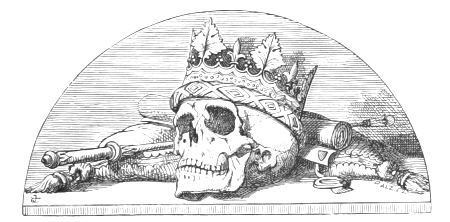
\includegraphics[scale=.5]{SkullLine}
  \end{center}



\MYSTERY [
  Name = Gaze of the Void,
  Link = arcana-mystery-gaze-of-the-void,
  Paradigm = Entropy,
  Save = Y (neg.),
  Duration = Instant,
  Target = Nearby or Far-Away Target(s)
]

A Monster disintegrates into nothingness. The number of \DICE invested must be twice the Monster's \HD + 1 (for example, to disintegrate a 1 \HD creature, you must invest 3 \DICE (1x2+1), a 2 \HD requires 5 \DICE, etc.) Monsters get a +2 to their Save; magical objects and magical monsters (dragons, unicorns, etc) get a +4 to their Save.



\MYSTERY [
  Name = Kismet,
  Link = arcana-mystery-kismet,
  Paradigm = Entropy,
  Save = n/a,
  Duration = Session,
  Target = See Below
]

Take \DICE Faith and put them "in reserve".  For the remainder of the Session, you may roll one of these [die] to modify \myital{any} \RO or \RB roll (by Ally or Monster alike) either plus or minus the \SUMDICE of the die roll.  You can only use 1 [die] per roll.  Regardless of the \SUMDICE of the [die], the Faith die is lost the moment it is rolled.  Any unused \DICE are lost at the end of the Session.  You can only invoke this mystery once per Session.

\MYSTERY [
  Name = Limbbreaker,
  Link = arcana-mystery-limbbreaker,
  Paradigm = Biomancy,
  Save = Y (neg.),
  Duration = Markovian,
  Target = Far-Away Target(s)
]

The target of this spell must have limbs.  With a snap of the fingers, \DICE of the target's limbs bend, crack, and break.  If an arm is broken, anything held in the hand is immediately dropped; if a leg is broken, the creature falls Prone; if both arms are broken, nothing can be picked up (and no spells can be cast); if both legs are broken, the Monster can only crawl.  The limbs remain broken for the Markovian duration, after which they immediately heal with no ill effects. Save negates.  Note that this spell can only target Far-Away creatures.

\MYSTERY [
  Name = Shrikeblast,
  Link = arcana-mystery-shrikeblast,
  Paradigm = Force,
  Save = Y (half),
  Duration = Instant,
  Target = Far-Away Target(s)
]

You let out a scream which shatters into shards of force.  The shards can lacerate up to \DICE  Far-Away Monsters and deal \SUMDICE+\DICE total damage (divided up any way you want).  If a Monster is killed by this spell, it will be suspended in the position it was killed for \SUMDICE Minutes by by the shards. A suspended creature is capable of bearing up to its own body weight in additional pressure before falling.  Note that this spell can only target Far-Away creatures.

\MYSTERY [
  Name = Storm of Hammers,
  Link = arcana-mystery-storm-of-hammers,
  Paradigm = Force,
  Save = Y (half),
  Duration = Concentration,
  Target = Far-Away Target(s)
]

Invisible hammers of Force strike up to \DICE Monsters from every direction.  Target Monsters take \DICE Bashing damage each, depending on how you split the die (Save for half).  The liturgy lasts for as long as you Concentrate.  Concentration and spell-casting is impossible while being struck by these hammers. Note that this spell can only target Far-Away creatures.

\MYSTERY [
  Name = Vermin Swarm,
  Link = arcana-mystery-vermin-swarm,
  Paradigm = Biomancy,
  Save = n/a,
  Duration = Concentration,
  Target = Close or Nearby
]

You summon a swarm of vermin that crawl up from the ground, walls, and ceiling.  The swarm can be directed for as long as you Concentrate and have a Base Speed (d16, 2 Maneuvers).  The swarm has \SUMDICE Health and deals \DICE damage to all Monsters Close to them provided a successful Fight roll is made (roll your \FOC for your Fight check).  Swarms take double damage from attacks that affect multiple targets, and share their Health equally as one "pool".  

\MYSTERY [
  Name = Wall of Gloom,
  Link = arcana-mystery-wall-of-gloom,
  Paradigm = Mind,
  Save = See Below,
  Duration = Markovian,
  Target = Nearby or Far-Away
]

You can anchor a barrier of pure darkness between three or more solid points up to \DICE meters in radius (for example: the 4 points of a door, two trees and the ground, across a hallway, etc).  Monsters that touch the blackness must immediately make a morale check with a -\DICE penalty or become Afraid for a Markovian duration.  If you spend 3 or more Faith, creatures that make their morale check that then continue through the wall must make a second Save; if they fail, they exit the wall the same way they came in (they will need to make a morale check again to touch the wall if they wish to try to move through it again).   

